\subsection{Workbench}\label{workbench}
De workbench biedt een handig overzicht voor (eind)redacteuren. Via de workbench kun je bijvoorbeeld makkelijk bekijken welke inhoud recentelijk is aangemaakt of welke inhoud nog beoordeeld moet worden.

\subsubsection{Workbench overview}\label{workbenchoverview}
De onderstaande afbeelding toont de Workbench. 
\bigskip

\begin{center}
	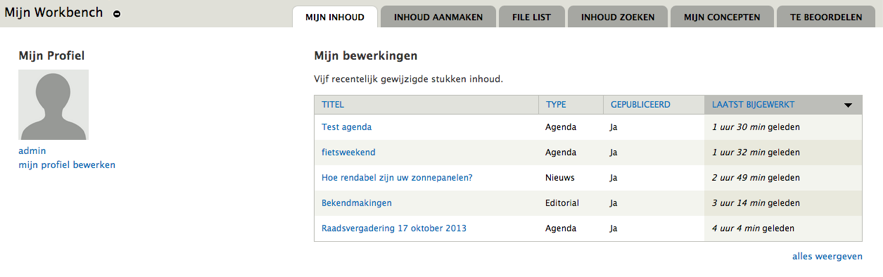
\includegraphics[width=\textwidth]{img/workbench.png}
\end{center}

\textbf{Mijn inhoud:} toont de inhoud welke recentelijk is bewerkt door de gebruiker .

\textbf{Inhoud toevoegen:} link naar de pagina 'Inhoud toevoegen'.

\textbf{File list:} toont alle bestanden welke recentelijk zijn toegevoegd.

\textbf{Inhoud zoeken:} link naar de pagina 'Inhoud zoeken', hier kun je gemakkelijk met behulp van filters op inhoud zoeken.

\textbf{Mijn concepten:} toont alle concepten aangemaakt door de gebruiker 

\textbf{Te beoordelen:} toont alle content items welke nog goedgekeurd moeten worden door de eindredacteur.

\subsubsection{Workbench workflow}\label{workbenchworkflow}

De workflow binnen de workbench gaat als volgt. Een redacteur voert nieuwe content op als 'concept'. Zolang het een concept blijft zal deze terug te vinden zijn onder de tab 'Mijn concepten'. Dit item zal dan niet aan de voorkant te lezen zijn. De redacteur kan dan kiezen om het ter beoordeling aan te bieden. Het item zal dan verschijnen onder de tab 'Te beoordelen' van een gebruiker met de rol 'eindredacteur'. De eindredacteur kan dan kiezen om het item terug te zetten naar concept of om het te publiceren. 

Bij het bewerken van bestaande content geldt dezelfde flow. Van het bestaande item zal dan een nieuw concept gemaakt worden, wat door de redacteur ter beoordeling aangeboden kan worden. Om daarna door een eindredacteur te publiceren of terug te zetten naar concept.